\chapter{Datasets and Evaluation}\label{ch:datasets}
Every problem to be solved with machine learning and data mining techniques
requires the availability of data for algorithm parametrization: the ability to
access public dataset, representative of a real scenario, allows to test the approaches, in order to evaluate the effective benefit in real applications, and
to compare the performance of existing approaches on a common comparison
basis. A reliable
evaluation procedure for a classification or recognition system will involve a
standard dataset of example input data along with the intended target output, and
well-defined metrics to compare the systems’ outputs with this ground truth. 

%TODO Define typical characteristics of dataset acquisition

\section{Datasets for Sound Event Detection}
In order to evaluate the proposed method in polyphonic real-life conditions, we used the TUT Sound Events 2016 \& 2017 datasets, which were included in the corresponding editions of the DCASE Challenge. For the monophonic-SED case study, we used the TUT Rare Sound Events 2017 which represents the task 2 of the DCASE 2017 Challenge.

\subsubsection{TUT Sound Events 2016}
The TUT Sound events 2016 (TUT-SED 2016)\footnote{\url{http://www.cs.tut.fi/sgn/arg/dcase2016/}} dataset consists of recordings from two acoustic scenes, respectively ``Home'' (indoor) and ``Residential area'' (outdoor) which we considered as two separate subsets. These acoustic scenes were selected from the challenge organizers to represent common environments of interest in applications for safety and surveillance (outside home) and human activity monitoring or home surveillance \cite{mesaros2016tut}.
%The dataset was collected in Finland by Tampere University of Technology from different locations by means of a binaural recording system. For each location, a 3-5 minute long binaural
%audio recording is provided for a total of around 54 and 59 minutes of audio respectively for ``Home'' and ``Residential area'' scenario.
A total amount of around 54 and 59 minutes of audio are provided respectively for ``Home'' and ``Residential area'' scenarios.
Sound events present in each recording were manually annotated without any further cross-verification, due to the high level of subjectivity inherent to the problem. 
For the ``Home'' scenario a total of 11 classes were defined, % (including Object impact, People walking, Washing dishes),
while for the ``Residential Area'' scenario 7 classes were annotated. % (including Bird singing, Car passing by, People speaking).

Each scenario of the TUT-SED 2016 has been divided into two subsets: development dataset and evaluation dataset. The split was done based on the number of examples available for each sound event class. In addition, for the development dataset a cross-validation setup is provided in order to easily compare the results of different approaches on this dataset. The setup consists of 4 folds, so that each recording is used exactly once as test data. In detail, ``Residential area'' sound events data consists of 5 recordings in the evaluation set and 12 recordings in the development set while ``Home'' sound events data consists of 5
recordings in the evaluation set and 10 recordings in turn divided into 4 folds as training and validation subsets.


\subsubsection{TUT Sound Events 2017}
The TUT Sound Events 2017 (TUT-SED 2017)\footnote{\label{note_dcase17}\url{http://www.cs.tut.fi/sgn/arg/dcase2017/}} dataset consists of recordings of street acoustic scenes with various levels of traffic and other activities, for a total of 121 minutes of audio. The scene was selected as representing an environment of interest for detection of sound events related to human activities and hazard situations. It is a subset of the TUT Acoustic scenes 2016 dataset \cite{mesaros2016tut}, from which also TUT-SED 2016 dataset was taken. Thus, the recording setup, the annotation procedure, the dataset splitting, and the cross-validation setup is the same described above. The 6 target sound event classes were selected to represent common sounds related to human presence and traffic, and they include brakes squeaking, car, children, large vehicle, people speaking, people walking. The evaluation set of the TUT-SED 2017 consists of 29 minutes of audio, whereas the development set is composed of 92 minutes of audio which are employed in the cross-validation procedure.

\subsubsection{TUT Rare Sound Events 2017} 
The TUT Rare Sound Events 2017 (TUT-Rare 2017)\textsuperscript{\ref{note_dcase17}} \cite{DCASE2017challenge} consists of isolated sounds of three different target event classes (respectively, baby crying, glass breaking and gunshot) and 30-second long recordings of everyday acoustic scenes to serve as background, such as park, home, street, cafe, train, etc. \cite{mesaros2016tut}. In this case we consider a \textit{monophonic}-SED, since the sound events are artificially mixed with the background sequences without overlap. In addition, the event potentially present in each test file is known a-priori thus it is possible to train different models, each one specialized for a sound event. In the development set, we used a number of sequences equal to 750, 750 and 1250 for training respectively of the baby cry, glass-break and gunshot models, while we used 100 sequences as validation set and 500 sequences as test set for all of them. In the evaluation set, the training and test sequences of the development set are combined into a single training set, while the validation set is the same used in the Development dataset. The system is evaluated against an ``unseen'' set of 1500 samples (500 for each target class) with a sound event presence probability for each class equal to 0.5.

\subsection{Snore Sound Detection in Real Life Audio}
\label{ssec:dataset}
The snore detection algorithm has been evaluated on the A3-Snore dataset. A brief description of the acquisition setup and dataset splitting is provided in the following.

\subsubsection{Acquisition setup:}
In order to capture the overnight audio recordings a ZOOM-H1 Handy Recorder has been used. It is equipped with two unidirectional microphones set at a 90 degree angle relative to one another. The signals are stored in WAV files with a sampling rate of 44.1\ kHz and bit depth equal to 16.
The input gain is automatically set by the recorder to prevent overload and distortion, while the high-pass filter was enabled in order to eliminate pops, wind noise, blowing, and other kinds of low frequency rumble.


\subsubsection{Acquisition environment:}
The acquisition environment consist of a simple bedroom, with two access points (door and window). The recorder is placed near the patient, at same height of the bed and in line with the subject's mouth. During the recordings, the patient is the only one that can occupy the bedroom, in order to avoid contaminations on recorded audio signals. The room dimensions are reported in \figref{fig:room}.
Background sounds include traffic noise, breathing and speech signals, house and animal noises. We acquired some samples measurements of the event-to-background (EBR) ratios considering background noise, snoring events and noise events such as ``car passing by'' or ``dog barfing''. The EBR resulted equal to 6.5 dB and 1.1 dB respectively for noise to background EBR and snore to background EBR. 


\begin{figure}[t]
	\centering
	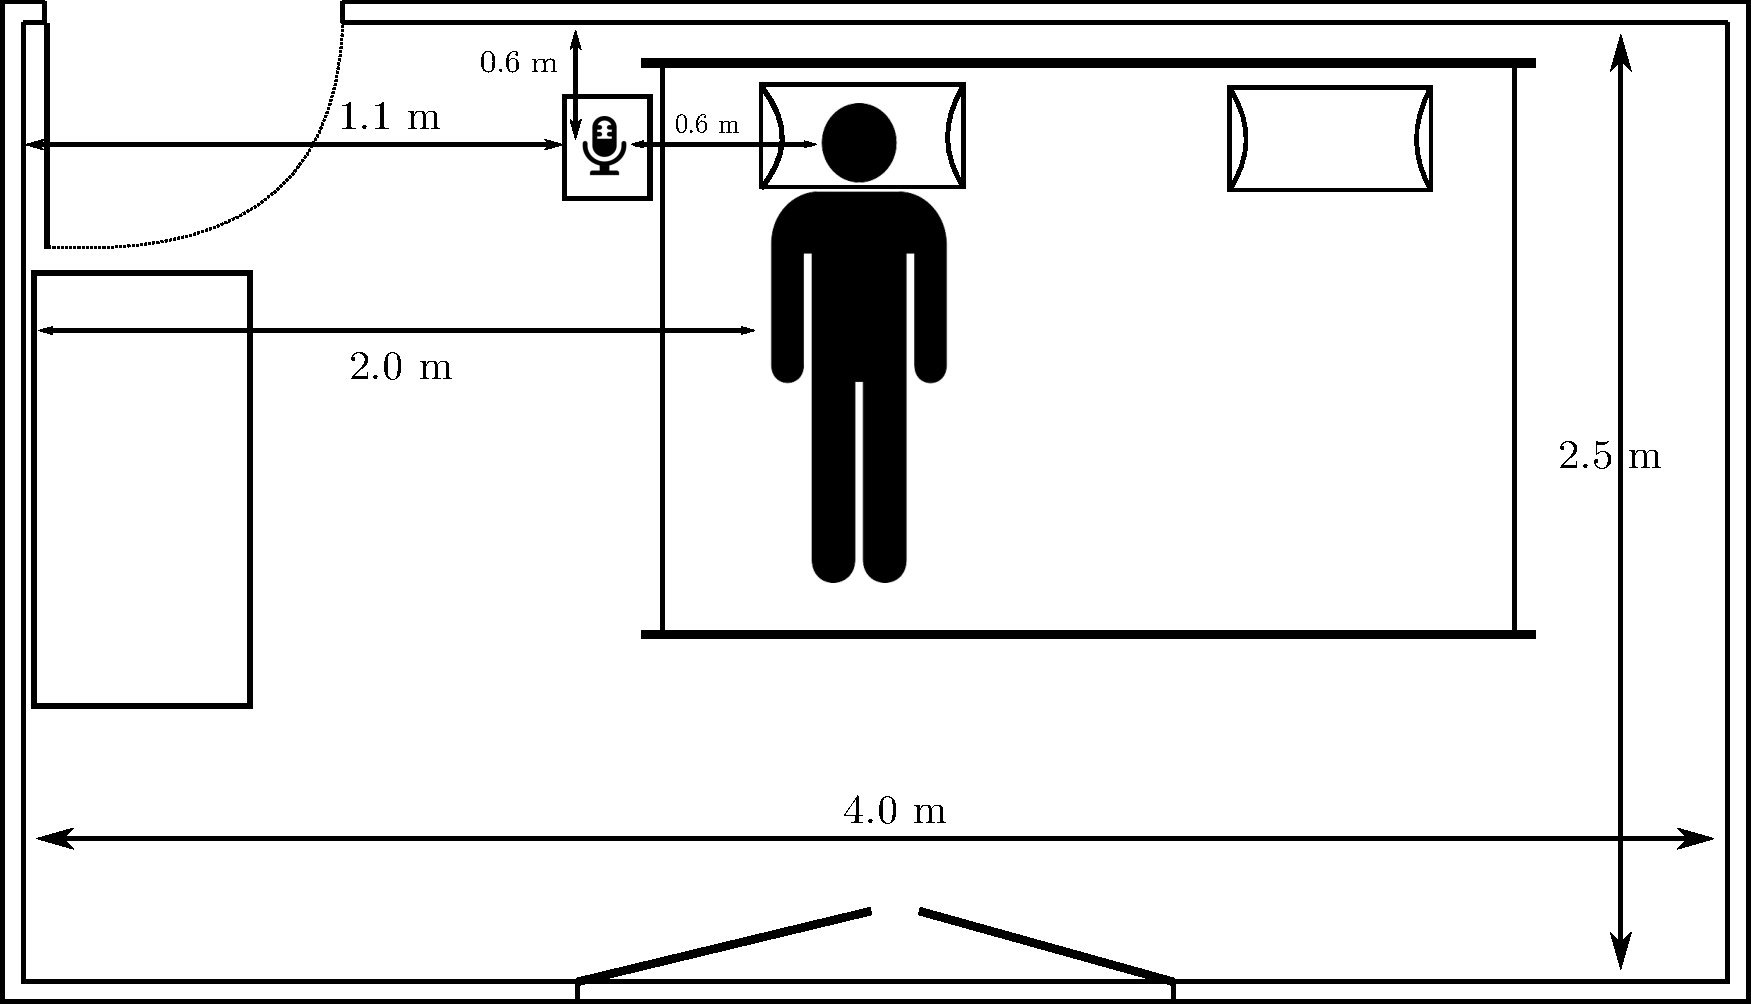
\includegraphics[width=0.8\columnwidth]{img/room.pdf}
	\caption{Plant of the recording room.} 
	\label{fig:room}
\end{figure}


\subsubsection{Dataset splitting:}
The original recordings have been manually labelled, annotating the snore events onset and offset with a resolution of 1 second. The audio sequences have been divided into chunks of 10 minutes, and only those with the highest number of snore events have been used in the experiments. 
The dataset is organized into subjects, which can be respectively used as \emph{training} or \emph{validation} sets in a two fold cross validation strategy (i.e., Leave One Subject Out procedure). The number of events per class in the database is strongly unbalanced as reported in \tableref{a3snore}. Thus, the snore detection task is challenging, due to the high number of noises on the A3-SNORE dataset. 

\begin{table}[ht]
	\centering
	\caption[A3-SNORE dataset]{Difference of recording times for each class, divided by snorers.}
	\begin{tabular}{cccccc}
		\hline
		\multicolumn{6}{c}{\textbf{A3-SNORE dataset}} \\
		\hline
		\# & Gender & Age & Snoring (SN) & Total Duration (Tot) & Ratio (SN/Tot) \\
		\hline
		Snorer 1 & M & 48 & 33m-27s & 3h-12m-0s & 14.5\% \\
		Snorer 2 & M & 55 & 21m-21s & 3h-50m-0s & 11.1\% \\
		\hline
		\multicolumn{3}{l}{Total} &	54m-48s	& 7h-02m-0s	& 12.8\%\\
		\hline    
	\end{tabular}	
	\label{a3snore} 
\end{table}

\subsection{Acoustic Novelty Detection}

\label{sec:databases}
This section describes the three databases evaluated in our experiments: A3Novelty, PASCAL CHiME, and PROMETHEUS.

\subsubsection{A3NOVELTY}

%FABIO Description of A3Corpus taken from ESWA paper. Io l'ho parafrasata in modo "light"...vedete voi se bisogna modificarla di più.

%TODO: add description of the database.

%TODO: add final table including stats on the datasets (number of abnormal sounds, duration etc...


The A3Novelty corpus\footnote{\label{note:a3}\url{http://www.a3lab.dii.univpm.it/research/a3novelty}} includes around 56 hours of recording acquired in a laboratory of the Università Politecnica delle Marche. 
These recordings were performed during different day and night hours, so very different acoustic conditions are available.
A variety of \emph{novel} events were randomly played back by a speaker (e.g., scream, fall, alarm or breakage of objects) during the recordings.

Eight microphones were used in the recording room for the acquisitions: four Behringer B-5 microphones with cardioid pattern and an
array of four AKG C400 BL microphones spaced by 4\,cm, then A MOTU 8pre sound card and the NU-Tech software were utilised 
to record the microphone signals. The sampling rate was equal to 48\,kHz.


The abnormal event sounds (cf.  Table \ref{tab:events}) can be grouped into four categories and they are freely available to download from \url{http://www.freesound.org}:
\begin{itemize}
	\item \textit{Sirens}, three different types of sirens or alarm sounds.
	\item \textit{Falls}, two occurrences of a person or an object falling to the ground.
	\item \textit{Breakage of objects}, noise produced by the breakage of an object after the impact with the ground.
	\item \textit{Screams}, four different human screams, both produced by a single person or by a group of people.
\end{itemize}


The A3Novelty corpus is composed of two types of recordings:
\emph{background}, which contains only background sounds such as human speech, technical tools noise and environmental sounds and \emph{background with novelty}, which contains in addition to the background the artificially generated novelty events.

In the original A3Novelty database the recordings are segmented in sequences of 30 seconds. In order to limit the size of training data, we randomly selected 300 sequences from the \emph{background} partition to compose of training material (150 minutes), and 180 sequences from the \emph{background with novelty} partition to compose the testing set (90 minutes). The test set contains 13 novelty occurrences.

For reproducibility, the list of randomly selected recordings, as well as the train and test set are made available % \footnotemark[\ref{note:a3}]. %ndFAB\footnotemark [3].


%\begin{table}[t]
%\centering
%\begin{tabular}{lccc}
%\hline
%\textbf{Rec Type} & \textbf{Day/Night} & \textbf{Length (hh:mm)} & \textbf{Novelty events}\\
%\hline
%\multirow{2}{*}{Background} & Day & 12:00 & -\\
%& Night & 24:00 & -\\
%\hline
%Background & Day & 9:00 & 16\\
%with novelty & Night & 12:00 & 30\\
%\hline
%\end{tabular}
%\caption{Recordings details.}
%\label{tab:recs_detail}
%\end{table}


\subsubsection{PASCAL CHiME}
\label{subsec:pascal}

The original dataset is composed of around 7 hours of recordings of a home environment, taken from the PASCAL CHiME speech separation and recognition challenge \cite{barker2013pascal}. 
It consists of a typical in-home scenario (a living room), recorded during different days and times,
while the inhabitants (two adults and two children) perform common actions, such as talking, watching television, playing, or eating. The dataset was recorded in stereo (with a binaural microphone) and a sample-rate of 16\,kHz. In the original PASCAL CHiME database the recordings are segmented in sequences of 5 minutes duration. In order to limit the size of training data, we randomly selected sequences to compose 100 minutes of background for the training set, and around 70 minutes for the testing set. For reproducibility, the list of randomly selected recordings, as well as the train and test set are made available\footnote{\url{http://a3lab.dii.univpm.it/webdav/audio/Novelty_Detection_Dataset.tar.gz}}. 
%The test set was generated adding different kinds of sounds\footnote{taken from www.freesound.org}, such as screams, alarms, falls and fractures (cf.\ Table \ref{tab:events}). 
%The test set did not include any overlapping events, the events were  and they were added at random position thus the distance between one event and another is not fixed. %ndFAB\footnotemark [1].
% %VES
The test set was generated adding different typologies of sounds\footnote{taken from www.freesound.org}, such as screams, alarms, falls and fractures (cf.\ Table \ref{tab:events}), after their normalization to the volume of the background recordings. % %
The events in the test set were added at random position (avoiding overlapping), thus the distance between one event and another is not fixed. %ndFAB\footnotemark [1].




\subsubsection{PROMETHEUS}
\begin{table}[t]
	\centering
	\tabcolsep=0.10cm
	\renewcommand{\arraystretch}{1.0}
	\caption[Acoustic novel events]{Acoustic novel events in the test set. Shown are the number of different events per database, the average duration, and the total duration in seconds per event type. The last column indicates the total number of events and total duration across the databases. The last line indicates the total duration in seconds of the test set including normal and novel events per database.}
	
	\begin{tabular}{ l || c c || c c || c c | c c | c c | c c || c c }
		\textbf{Events} & \multicolumn{2}{|c||}{A3Novelty} & \multicolumn{2}{|c||}{PASCAL CHiME} & \multicolumn{8}{|c||}{PROMETHEUS} & \multicolumn{2}{|c}{Total}\\
		\textbf{} & \multicolumn{2}{|c||}{} & \multicolumn{2}{|c||}{} & \multicolumn{2}{|c|}{ATM} & \multicolumn{2}{|c|}{Corridor} & \multicolumn{2}{|c|}{Outdoor} & \multicolumn{2}{|c||}{Smart-room} & \multicolumn{2}{|c}{}\\
		\textbf{} & \# & time(avg.) & \# & time(avg.) & \# & time(avg.) & \# & time(avg.) & \# & time(avg.) & \# & time(avg.) & \# & time\\
		\hline
		Alarm			& - & -		& 76 & 435.8 (6.0) 	 				& - & -			& 6 & 84.0 (14.0)	& - & -				& 3 & 9.0 (3.0)		& 85 & 528.8\\
		Anger			& - & - 				& - & - 				& - & -			& - & -				& 6 & 293.0 (48.8)		& - & - 			& 6 & 293.0\\  
		Fall 			& 3 & 4.2 (2.1)		& 48 & 89.5 (1.8) 	& - & -	 		& 3 & 3.0 (1.0)		& - & -				& 2 & 2.0 (1.0) 		& 55 & 98.7\\
		Fracture		& 1 & 2.2 			& 32 & 70.4 (2.2) 	& - & - 			& - & -				& - & -				& - & - 				& 33 & 72.6\\
		Pain			& - & -			 	& - & - 			& - & -	 		& 2 & 8.0 (4.0)		& - & -				& 5 & 67.0 (13.4) 		& 7 & 75.0\\
		Scream			& 6 & 10.4(1.7)		& 111 & 214.6 (1.9) 	& 5 & 30.0 (6.0)	& 25 & 228.0 (9.1)	& 4 & 48.0 (12.0)		& 10 & 234.0 (23.4) & 159 & 762.2\\
		Siren			& 3 & 20.4 (6.8)		& - & - 				& - & - 			& - & -				& - & -				& - & -				& 3 & 18.1\\
		\hline
		Total			& 13 & 38.1 (2.9) & 267 & 810.3 (3.1) 	& 5 & 30.0 (5.0) 		& 36 & 323.0 (9.0) 	& 10 & 341.0 (34.1) 	& 20 & 312.0 (15.6) & 348 & 1848.4\\
		\hline\hline
		Test time & - & 5400.0 				& - & 4188.0 	& - & 750.0			& - & 960.0	& - & 1620.0				& - & 1020.0		& - & 13938.0\\
		
	\end{tabular}
	\label{tab:events}
\end{table}

The PROMETHEUS database \cite{ntalampiras:probabilistic} contains recordings of various scenarios designed to serve a wide range of real-world applications. The database includes: 1) a \textit{smart-room} indoor home environment including phases where a user is interacting with an automated speech-driven home assistant, 2) an outdoor public space consisting of \textit{a}) interaction of people with an \textit{ATM}, \textit{b}) an \textit{outdoor} security scenario in which people are waiting in front of a counter, and 3) an  indoor office \textit{corridor} scenario for security monitoring in standard indoor space. 
%The first one is intended to be representative of particular activities which take place inside an intelligent environment, including phases where the user is interacting with an automated speech-driven home assistant. As for the second setting, two scenarios with different scopes were captured: 1) ATM scenario, which included interactions of people with an ATM, and 2) security scenario, in which people in a queue are waiting for service in front of a counter and can be utilized as a general-purpose scenario with many applications (e.g., bank, airport, etc.). The third setting was used for security scenarios in a standard indoors space. 
These scenarios substantially differ in terms of acoustic environment. The indoor scenarios were recorded under quiet acoustic conditions, whereas the outdoor recordings were conducted in an open-air public area and contain non-stationary background noise.   
The smart-home scenario contains recordings of five professional actors performing five single-person and 14 multiple-person action scripts. The main activities include human-machine interaction with a virtual home agent, a number of alternating normal and abnormal activities specifically designed to monitor and interpret human behaviour. The single-person and multiple-person actions include abnormal events, such as: falls, alarm followed by panic, atypical vocalic reactions (pain, fear, anger), or fractures. Examples are: walking to the couch, sitting or interacting with the smart environment to turn the TV on, open the windows, or decrease the temperature. The scenarios were recorded three to five times, by changing the actors and their roles in the action scripts.
Table \ref{tab:events} provides details on the number of abnormal events per scenario, including average time duration.


\section{The DIRHA Dataset}
\label{sec:dataset}

\begin{figure}[h]
	\centering
	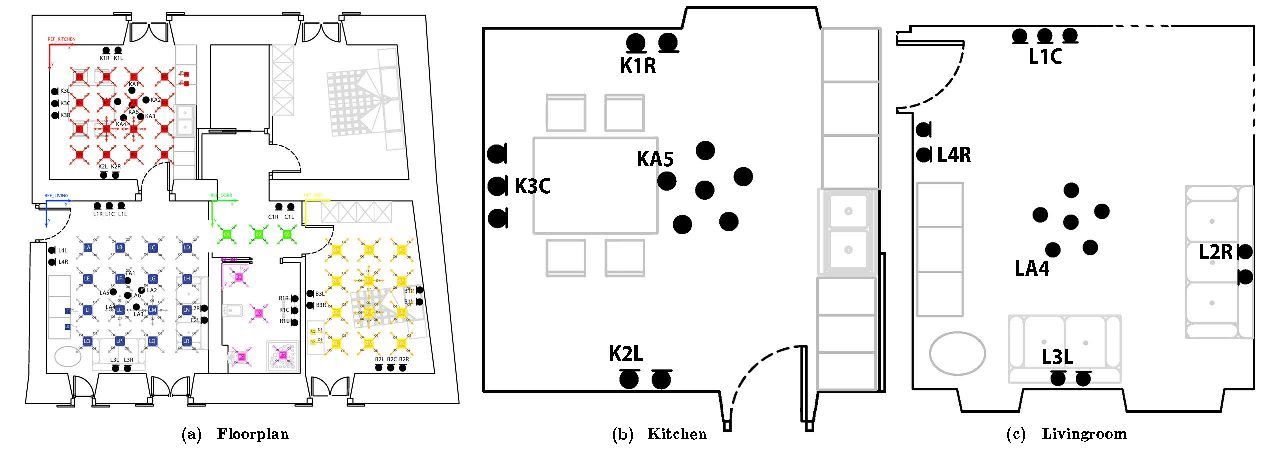
\includegraphics[width=\textwidth]{img/plan}
	\caption{The map of the apartment used for the DIRHA project (a). Figures (b) and (c) show the considered rooms, with the disposition of their relative microphones. }
	\label{fig:DIRHA_map}
\end{figure}

The analysis of the DNN-SLOC performance has been conducted on the DIRHA dataset \cite{cristoforetti2014dirha}, characterized by diverse scenes, rooms, microphones and noise conditions\footnote{\url{http://dirha.fbk.eu/simcorpora}}. In details, the apartment where the dataset has been recorded consists in five rooms and a total of 40 microphones. These are arranged in linear and circular arrays, with the first ones placed on the walls of all rooms, and the circular ones are placed on the ceiling of the living room and of the kitchen (\figref{fig:DIRHA_map}).

The dataset is composed of two subsets, named \emph{Simulated} and \emph{Real}. For each of them several \textit{scenes} have been recorded, composed of typical situations observable in a domestic context. As reported in \tableref{tab:dataset}, the two subsets differ in terms of scenes and total length: in the Simulated set the scenes length is fixed to 60 seconds, while it varies in the Real set. In addition, the latter has been recorded with persons moving in the rooms and speaking towards different directions throughout the scenes, whilst the Simulated has been obtained by convolving a fixed set of measured Room Impulse Responses (RIRs) with recorded signals.
The Simulated subset is also characterized by a lower SNR compared to the Real one and overlapping speech does not occur.

Our study focuses on two rooms of the dataset, i.e.,  the Kitchen and the Living Room, due to three main aspects. First of all, these rooms consist in the area of a home-environment where most of the events take place. In addition, being the widest rooms of the apartment, the localization task is more challenging. \textcolor{red}{The room dimensions are respectively $4.79$\,m~$\times$~$3.80$\,m for the Kitchen and $4.79$\,m~$\times$~$4.85$\,m for the Living Room.}
Finally, the number of microphones are higher compared to the other rooms, and they comprise both wall and ceiling arrays.

\begin{table}[t]
	%\renewcommand{\arraystretch}{1.2}
	\centering
	%	\small
	\caption{Main differences between the Real and Simulated subsets.}
	\resizebox{.75\columnwidth}{!}{%
		\begin{tabular}{c|c|c}\hline
			& \textbf{Real} & \textbf{Simulated} \\ \hline
			\textbf{Nr.\ of Scenes}  & 22 & 80 \\ \hline
			
			\textbf{Total Duration} &  21.5 min. & 80 min.  \\  \hline
			\multirow{2}{*}{\textbf{Speech Percentage}}	&  12.9\%  & 23.6\%  \\
			& 	2.8  min.	& 18.9 min. \\ \hline
			\textbf{Source} & human (moving) & loudspeaker (static) \\ \hline
			\textbf{Background} & quiet & various \\ \hline
			\textbf{Noise Source Rate} & low & high \\ \hline
			\textbf{Overlapping Events} & no & yes \\ \hline  
		\end{tabular} 
	}
	\label{tab:dataset}
\end{table}

\section{Datasets for Sound Event Classification}

\subsection{Acoustic Road Roughness Classification}
The dataset built for this work is done with a multi-channel microphone arrangement, with the prospect of conducting different assessments at once or to exploit microphone diversity to improve the classification. More specifically, two microphones have been placed close to the rear wheels, one in front of the front left wheel, one inside the engine compartment and two inside the cockpit, close to the driver head and close to the right passenger head. The rear wheel microphones have been placed off-axis, in order to avoid dirt from the wheel and protected by the wheelhouse to reduce the effect of wind. Figure \ref{fig:car-mic} shows the positioning of all microphones. External microphones are \textit{PCB Piezotronics} model 130A24. These are IP55 microphones and they have been protected with a melamine resin foam for sound absorption to reduce the effect of wind. The internal microphones are \textit{PCB Piezotronics} model 378C20. The front-right wheel has been excluded from recordings after first informal evaluations because it picked a large amount of engine noise with respect to the other microphones. The rear-right microphone, vice versa, was found to be the best choice because the noise from the engine was the lowest and it has been used for this first evaluation. The engine compartment microphone has been used to record the engine conditions for future use. In \figref{fig:car-rr-and-fl} are shown the images of the microphones installation. 

\begin{figure}[ht]
	\centering
	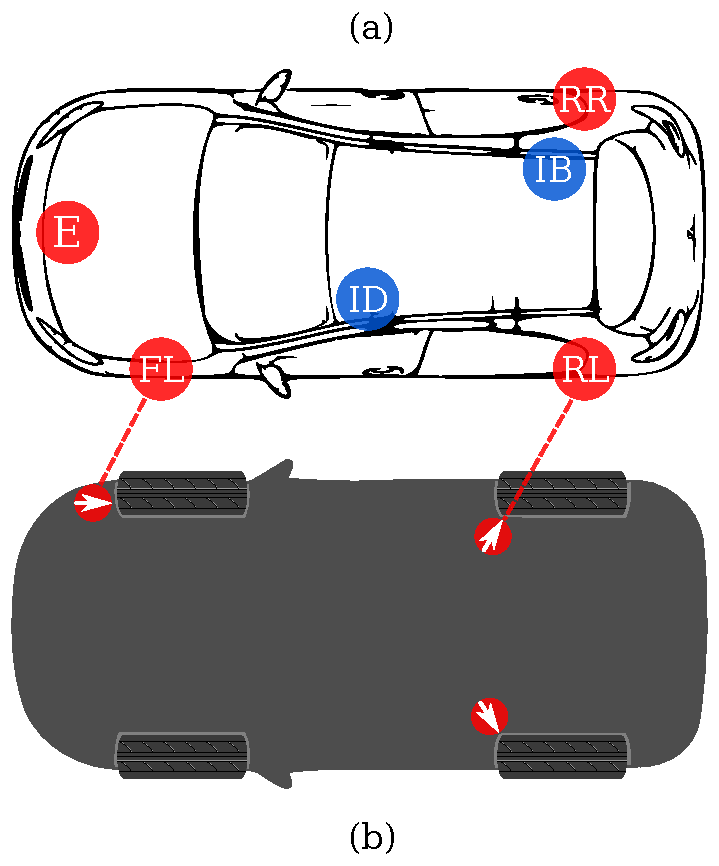
\includegraphics[width=0.5\textwidth]{img/car-mic}
	\caption[Position of the microphones in the car used to record the dataset]{Positioning of the microphones in the car used to record the dataset, top view (a) and bottom view (b). The microphones are placed in the engine compartment (E), close to the front-left, rear-left and rear-right tyres (FL, RL, RR), and inside the car close to the driver or in the back seat (ID, IB). The last two microphones are \textit{PCB Piezotronics} model 378C20 type microphones, while all the others are IP55 \textit{PCB Piezotronics} model 130A24 microphones. The microphones are omnidirectional, however the arrows in (b) show how the capsule was positioned to minimize wind effect. The rear microphones are protected in the wheelhouse.}
	\label{fig:car-mic}
\end{figure}

\begin{figure}[t]
	\centering
	\begin{subfigure}[b]{0.48\textwidth}
		\includegraphics[width=\textwidth]{img/Rear-Right.jpg}
		\subcaption{Rear right tyre microphone.}
	\end{subfigure}
	\hfil
	\begin{subfigure}[b]{0.48\textwidth}
		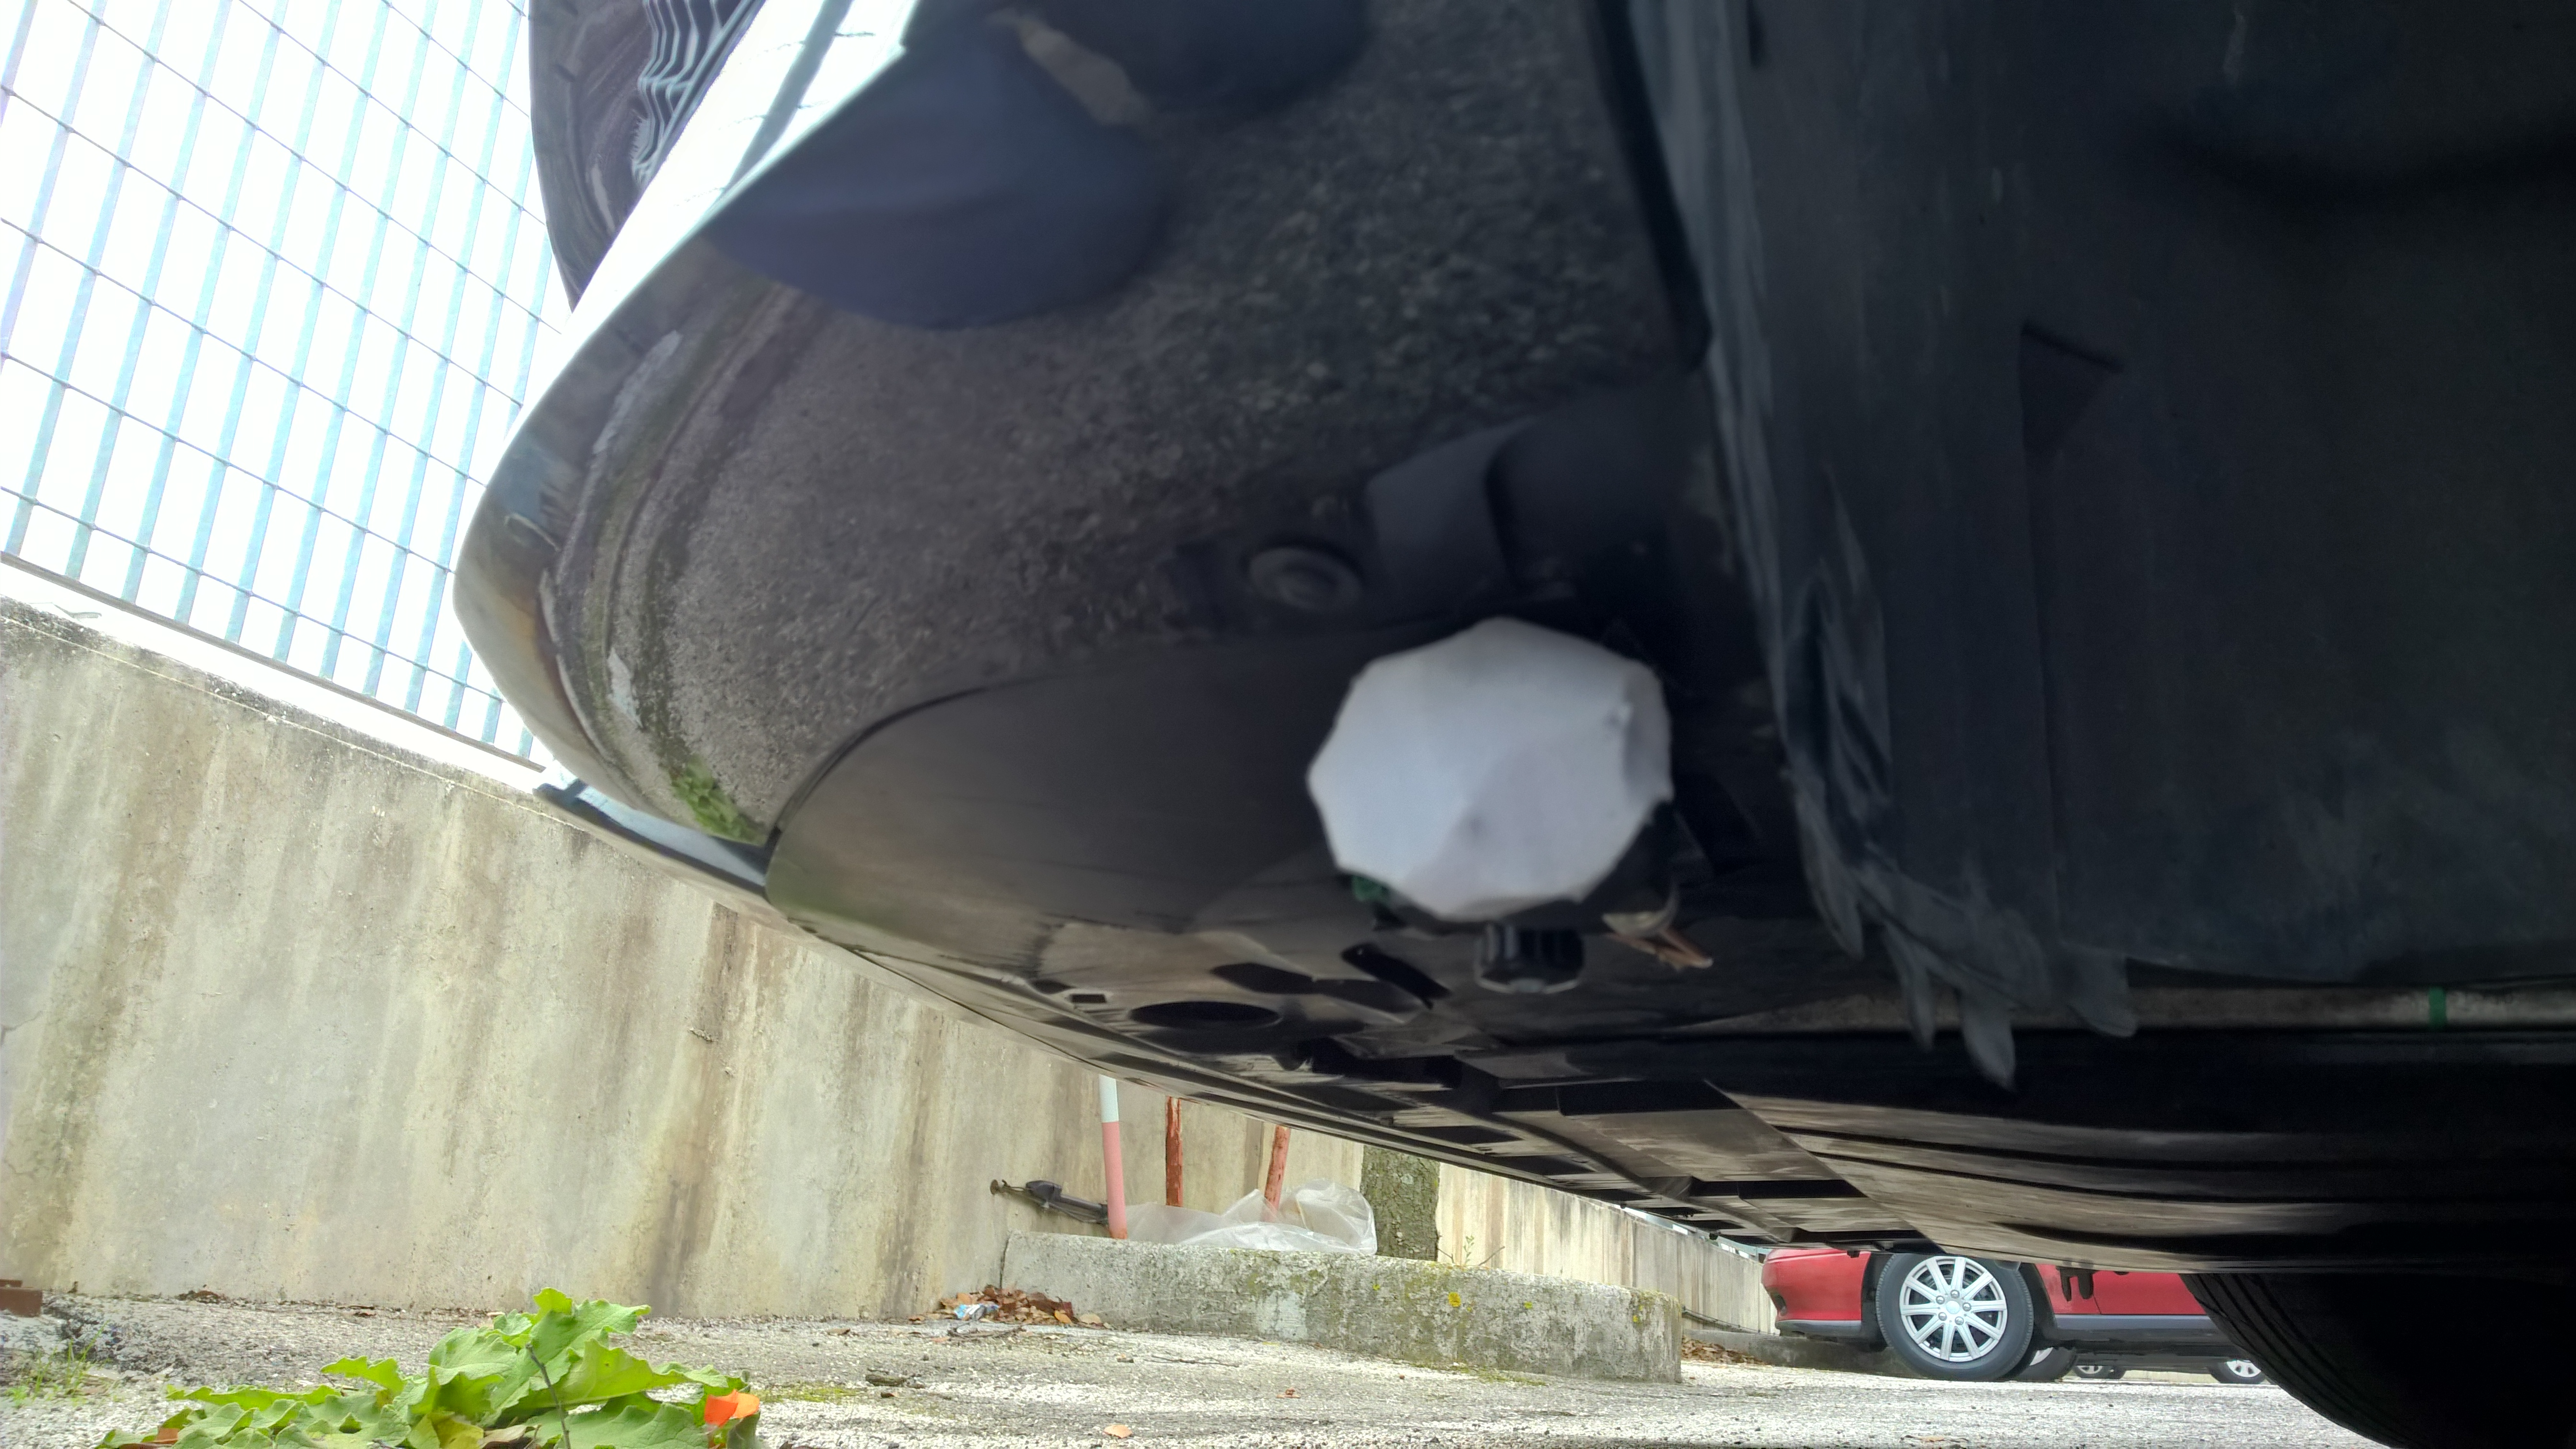
\includegraphics[width=\textwidth]{img/Front-Left.jpg}
		\subcaption{Front left tyre microphone.}
	\end{subfigure}
	
	
	\caption[\textit{PCB Piezotronics} model 130A24 microphones]{Pictures of the \textit{PCB Piezotronics} model 130A24 microphones positioned near the rear right and front left tyres, according to "RR" and "FL" red circles in \figref{fig:car-mic}. The microphones are enclosed by a melamine resin foam with open cell network structure to reduce the wind noise.}
	\label{fig:car-rr-and-fl}
\end{figure}



The car employed to build the dataset is Mercedes A Class from 2014. In addition to the audio signals, the GPS signal has been recorded to track down the car speed and position at any given time. A mobile multi-channel front end, \textit{HEAD Acoustics SQuadriga II}, has been employed as acquisition device, being able to monitor and record 8 contemporary channels at different sample rates, and to store GPS antenna and CAN bus signals.
All audio signals are sampled at 44100\,Hz, 24-bits. The external microphones used -26 dBV as input range while the interior microphones had -16 dBV as input range.
To facilitate the labelling operations, a camcorder \textit{BC Master DC10}\footnote{\url{http://www.bc-master.com/product/car-dash-camera-dc10}} was installed on the dashboard of the car. In addition to the video, it provides the speed information obtained through its own GPS antenna and it records the cockpit audio, useful for taking vocal notes while driving.

The data recorded with the \textit{HEAD Acoustics SQuadriga II} have been exported by means of the software \textit{HEAD Acoustics ArtemiS SUITE} in the uncompressed WAV audio format with a 32-bit float representation.

All recordings were taken in dry conditions in the urban and suburban areas of Ancona (Italy) with variable speed, traffic conditions and pavement roughness. Only roads that had been recently asphalted were considered and multiple takes at different speed for each road have been performed. The dataset is not perfectly balanced and is characterized by 41\% of rough road samples and 59\% of smooth road samples. For this reason a balanced version of the dataset, i.e. with equal number of smooth and rough samples, has been created by pruning excess samples for the most populated class. 
The result of the recording sessions is a 50-minutes-long dataset (41 minutes for the balanced version), with 6 audio channels and a speed channel. Labels for the roads have been annotated manually.

The spectrograms from two audio samples belonging to the smooth and rough classes are shown in Figure \ref{fig:spectrograms_road}.

\begin{figure}[ht]
	\centering
	\begin{subfigure}[b]{0.48\textwidth}
		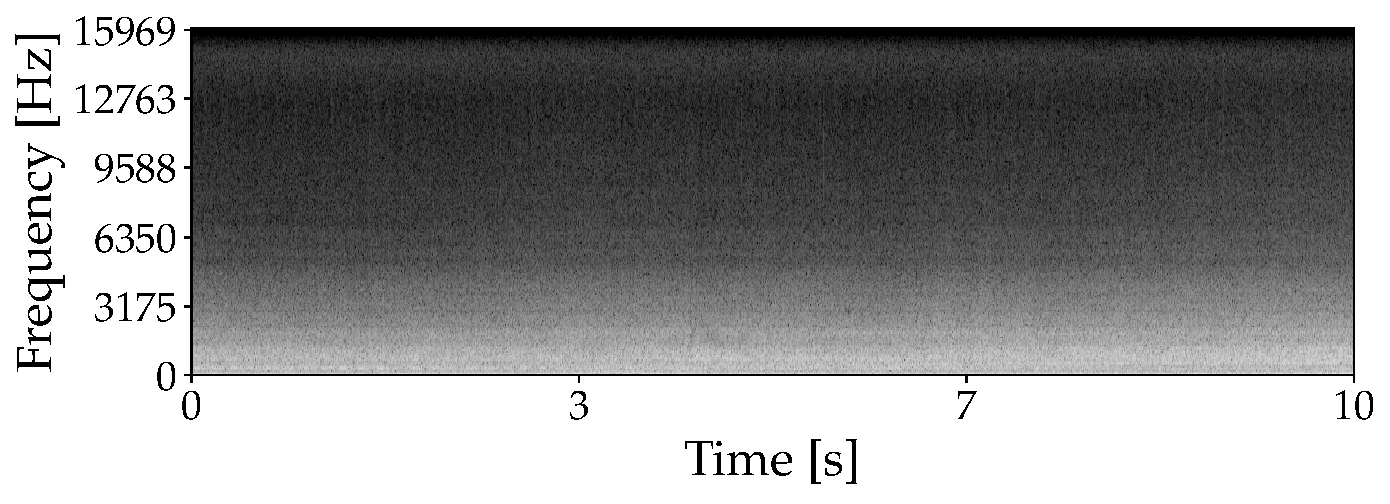
\includegraphics[width=\textwidth]{img/specgram_REC007}
		\subcaption{Smooth road.}
	\end{subfigure}
	\hfil
	\begin{subfigure}[b]{0.48\textwidth}
		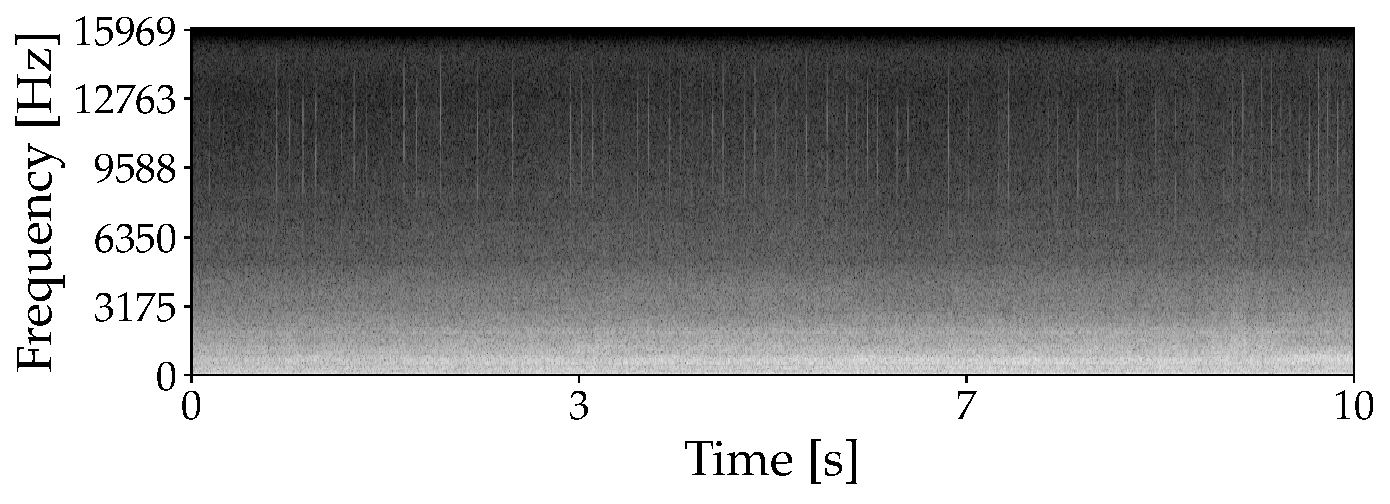
\includegraphics[width=\textwidth]{img/specgram_REC015}
		\subcaption{Rough road.}
	\end{subfigure}
	
	
	\caption[Spectrograms from 10 second samples]{Spectrograms from 10 second samples of (a) smooth urban road, (b) rough highway asphalt.}
	\label{fig:spectrograms_road}
\end{figure}

\subsection{Classification of Snore Sounds Excitation Locations}

\section{The MPSSC dataset}
\label{section:dataset}
The MPSSC dataset is composed of more than 30 hours of audio recordings captured during DISE examinations of 224 subjects from three medical centers recorded between 2006 and 2015. Recording equipment, microphone type, and location differ among the medical centers, so do the background noise characteristics. From the original signals (raw PCM, sample rate 16\,000\,Hz, quantization 16 bit) 843 early identifiable, single site of vibration snore events have been extracted and manually screened from medical experts.
Following the 4-class VOTE scheme, each sound file in the dataset is labelled as V, O, T, E, depending on the tissue from which snore sound originates, as shown in \figref{fig:vote}. They are respectively:
\begin{itemize}
	\item (V) - Velum (palate), including soft palate, uvula, lateral
	velopharyngeal walls;
	\item (O) - Oropharyngeal lateral walls, including palatine tonsils;
	\item (T) - Tongue, including tongue base and airway posterior to the tongue base;
	\item (E) - Epiglottis.
\end{itemize}

\begin{figure}[t]
	\centering
	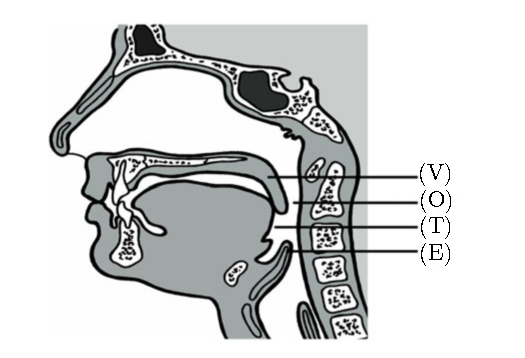
\includegraphics[width=0.6\linewidth]{img/vote.pdf}
	\caption[VOTE positions]{Corresponding positions of the VOTE classification in the upper airway. Picture courtesy of \cite{janott2014akustical}.} 
	\label{fig:vote}
\end{figure}


The dataset is divided into three subsets: \textit{train}, \textit{devel} and \textit{test}.
The number of events per class in the database is strongly unbalanced with a high preeminence of the ``Velum'' (V)-class  and ``Oropharyngeal'' (O)-class (85\% of samples) but in line with the likelihood of occurrence during normal sleep, while 10\% and 5\% of samples respectively belongs to E-events and T-snores. Details of class occurrences are shown in Table I.

\begin{table}[t]
	\centering
	\begin{tabular}{cccc}
		\toprule
		\multicolumn{4}{c}{\textbf{The Munich-Passau Snore Sound Corpus}} \\
		\midrule
		\#  \rule{10pt}{0pt}	& train  \rule{10pt}{0pt} & devel & test\\
		\midrule
		V \rule{10pt}{0pt}	& 168  \rule{15pt}{0pt} & 161 & 155\\
		O \rule{10pt}{0pt}	& 76  \rule{15pt}{0pt} & 75 & 65\\
		T \rule{10pt}{0pt}	& 8  \rule{15pt}{0pt} & 15 & 16\\
		E \rule{10pt}{0pt}	& 30  \rule{15pt}{0pt}& 32 & 27\\
		\bottomrule
		$\Sigma$  \rule{10pt}{0pt} & 282  \rule{13pt}{0pt} & 283 & 263\\
	\end{tabular}
	\caption[The Munich-Passau Snore Sound Corpus]{The Munich-Passau Snore Sound Corpus - The table shows the number of events per class in train, devel and test.}
	\label{tab:mpssc} 
\end{table}

%\begin{figure*}[t]
%	\centering
%	\includegraphics[width=\linewidth]{imgs/spectr-vote.png}
%	\caption{Waveforms and spectrograms of VOTE events}{(a) V (velum); (b) O (oropharyngeal); (c) T (tongue base); (d) E (epiglottis). \textbf{Rifare in HD, eventualmente aggiungere SCAT plot}} 
%	\label{fig:spectrograms}
%\end{figure*}


\begin{figure*}[t]
	\centering
	\begin{subfigure}{.40\textwidth}		
		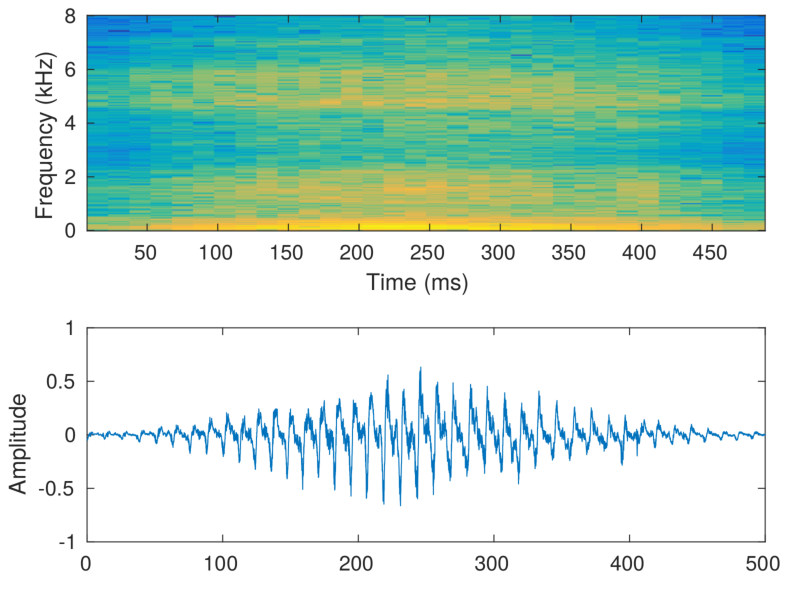
\includegraphics[width=0.9\linewidth]{img/V_spec_crop.pdf}
		\caption{}
		\label{fig:V}
	\end{subfigure}
	\begin{subfigure}{.4\textwidth}
		%\centering
		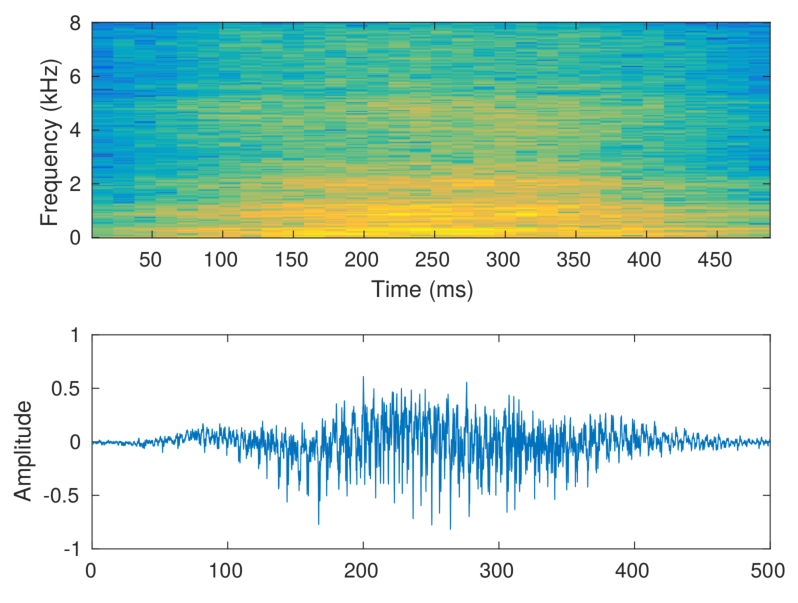
\includegraphics[width=0.9\linewidth]{img/O_spec_crop.pdf}
		\caption{}
		\label{fig:O}
	\end{subfigure}
	\begin{subfigure}{.40\textwidth}
		%\centering
		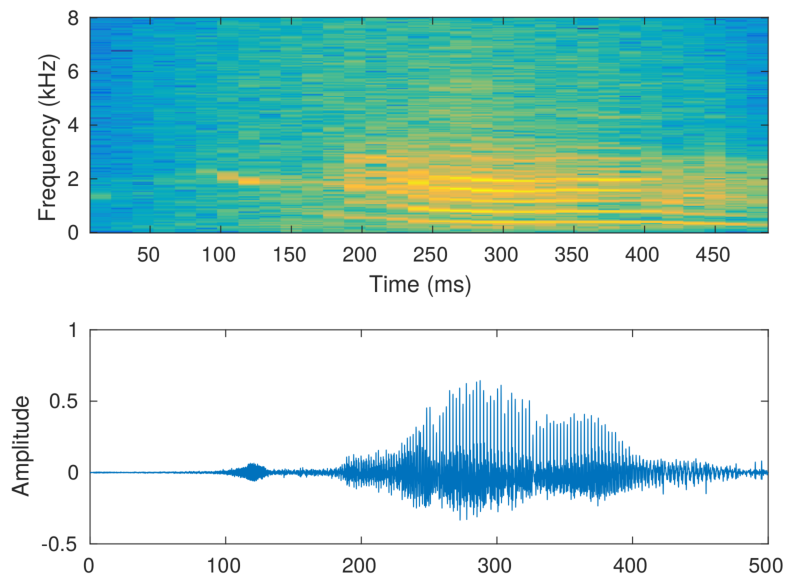
\includegraphics[width=0.9\linewidth]{img/T_spec_crop.pdf}
		\caption{}
		\label{fig:T}
	\end{subfigure}
	\begin{subfigure}{.40\textwidth}
		%\centering
		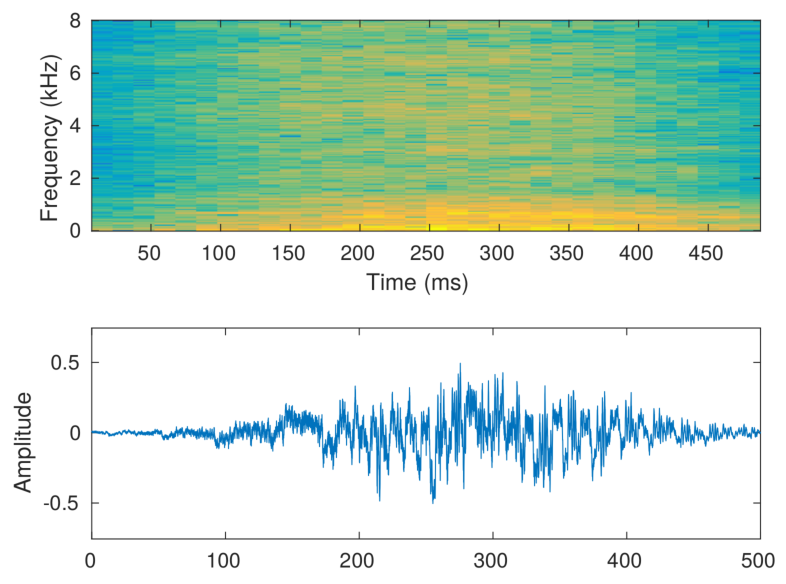
\includegraphics[width=0.9\linewidth]{img/E_spec_crop.pdf}
		\caption{}
		\label{fig:E}
	\end{subfigure}
	\caption{Waveforms and spectrograms of VOTE events}{(a) V (velum); (b) O (oropharyngeal); (c) T (tongue base); (d) E (epiglottis).}
	%\caption{Scat spectrum of VOTE events.  The top image is made of first-order coefficients, organized in a time-scale matrix. at the bottom of the image appear very low frequencies. The second-order coefficients for a fixed scale $m_1$, are shown in the bottom image, again in a time-scale matrix.}{(a) V (velum); (b) O (oropharyngeal); (c) T (tongue base); (d) E (epiglottis).}
	\label{fig:spectrograms}
\end{figure*}
As shown in the waveforms and the related spectrograms in \figref{fig:spectrograms}, the main energy components in three of the classes are concentrated in the frequency area below around 2000 Hz. Energy and spectral distribution characteristics are similar, except for the Type T, which shows higher energy content above 2500 Hz compared to the other three.


\subsection{Bird Audio Detection}
%\label{ssec:dataset}
According to the DCASE 2018 guidelines, the performance of the proposed algorithm has been assessed firstly by using the development dataset for training and validation of the system. Then, a blind test on the provided evaluation dataset was performed with the models which achieved the highest performance and submitted to the organizers of the challenge. The complete dataset is composed of recordings belonging to five different collections. Further details are reported below: %Further details are reported in Table \ref{tab:dataset}.

\begin{itemize}
	\item ``freefield1010'': a collection of 7690 excerpts from field recordings around the world;
	\item ``warblrb10k'': a crowsourced dataset recorded with the \textit{Warblr}\footnote{https://www.warblr.co.uk/} smartphone app. It covers a wide distribution of UK locations and environments and includes weather noise, traffic noise, human speech and even human bird imitations; 8000 samples are used in the development dataset while a held-out set of 2,000 recordings from the same conditions is included in the evaluation split;
	\item ``BirdVox-DCASE-20k'': 20000 files containing remote monitoring flight calls collected from  recordings units placed near Ithaca, NY, USA during the autumn of 2015;
	\item ``Chernobyl'': dataset collected from unattended remote monitoring equipment in the Chernobyl Exclusion Zone (CEZ). A totoal of 6620 audio files cover a range of birds and includes weather, large mammal and insect noise sampled across various CEZ environments, including abandoned village, grassland and forest areas;
	\item ``PolandNFC'': 4000 recordings obtained from a project of monitoring of autumn nocturnal bird migration. They were collected every night, from September to November 2016 on the Baltic Sea coast, Poland, using Song Meter SM2 units with microphones mounted on 3–5 m poles.
\end{itemize}

\begin{table}[t]
	\centering
	\begin{tabular}{|c|c|c|}
		\hline
		\ \textbf{Collection} \rule{0pt}{10pt} & \textbf{N. of samples}  & \textbf{Balance} \\
		\hline
		\hline	
		\multicolumn{3}{|c|}{\textbf{Development Dataset}  \rule{0pt}{10pt}} \\ 
		\hline
		``warblrb10k'' & 8000 & 0.75 \\
		\hline
		``BirdVox-DCASE-20k'' & 20000 & 0.5 \\
		\hline
		``freefield1010'' & 7690 & 0.25 \\
		\hline
		
		Total 	& 35690	& 0.5 \\
		
		\hline
		\hline
		
		\multicolumn{3}{|c|}{\textbf{Evaluation Dataset}  \rule{0pt}{10pt}} \\ 
		\hline
		``warblrb10k\_test'' & 2000 & - \\
		\hline
		``Chernobyl'' & 6620 & - \\
		\hline
		``PolandNFC'' & 4000 & - \\
		\hline
		Total 	& 12620 & - \\
		\hline
	\end{tabular}
	\caption{Details of the dataset we used for the algorithm development. The table shows the number of audio files and the ratio between positive/negative samples (if available) of each used data collection.}
	\label{tab:dataset} 
\end{table}

The organizers recommended a 3-way cross-validation (CV) for the algorithms development, thus in each fold we used two sets for training and the other one as validation set in order to have scores comparable with the others challenge participant.

\section{Evaluation Metrics}
\label{sec:evaluation_metrics}
Evaluation is usually referred as estimating the performance of a system under test
when confronted with new data. For an objective evaluation, the system is fed
previously unseen data for which reference annotations are available. The system output is then compared to the reference to calculate measures of its performance.

What performance means and how it should be measured may vary depending
on the specifications and requirements of the developed system: We can measure
accuracy to reflect how often the system correctly classifies or detects a sound, or we can measure error rates to reflect how often the system makes mistakes. By using
the same data and the same methodology to evaluate different systems, a fair and direct comparison can be made of systems’ capabilities.

The metrics used in detection and classification of sound events include accuracy, precision, recall, F-scor, area under the curve (AUC) or error rate (ER). There is no metric universally good for every kind of algorithm, as they each reflect different perspectives on the ability of the system.

\subsection{Metrics Computation}
Basically, the evaluation metrics are computed by comparing the prediction of the system under analysis with the respective annotations or \textit{ground truth}. Thus, the metrics are calculated based on counts of the correct predictions and different types of errors made by the system.
These counts are referred to as intermediate statistics and are defined depending on the evaluation procedure. These intermediate statistics are defined as follows for a target sound event:

\begin{itemize}
	\item True positive: A correct prediction, meaning that the system output and the reference both indicate the event present.
	\item True negative: The system output and the reference both indicate event not present.
	\item False positive: The system output indicates event  present or active, while the reference indicates event not present.
	\item False negative: The system output indicates event not present or inactive, while the reference indicatesit as present.
\end{itemize}

Sound event classification is usually a single-label multiclass problem, and the resulting intermediate metrics reflect whether the single true class is correctly recognized for each example. In this task there is no distinction between false positives and false negatives. 
In sound event detection, the choice of measurement determines the interpretation of the result: With a segment-based metric, the performance shows how well the system correctly detects the temporal regions where a sound event is
active; with an event-based metric, the performance shows how well the system is able to detect event instances with correct onset and offset. Thus, in the segment-based metric the ground truth and system output are compared in a fixed time grid, and sound events are marked as active or inactive in each segment. For the event-based metric the ground truth and system output are compared at event instance level. Specifically, the intermediate statistics for sound event detection are defined as follows:

\begin{itemize}	
	\item Substitutions $S$: are the number of ground truth events for which we have a false positive and one false negative in the same segment; %, thus: $S(t_1) = \min(FN(t_1),FP(t_1))$;	
	\item Insertions $I$: are events in system output that are not present in the ground truth, thus the false positives which cannot be counted as substitutions;%: $I(t_1) = \max(0,FN(t_1)-FP(t_1))$;
	
	\item Deletions $D$: are events in ground truth that are not correctly detected by the system, thus the false negatives which cannot be counted as substitutions;%: $D(t_1)= \max(0,FP(t_1)-FN(t_1))$.	
\end{itemize}

If we consider the scenario of polyphonic sound event detection, the segment-based metric essentially
splits the duration of the test audio into fixed length segments that have multiple associated labels, reflecting the sound events active anywhere in the given segment. In this respect, evaluation verifies if the system output and reference coincide in the assigned labels, and the length of the segment determines the temporal resolution of the evaluation. 
Event-based metrics compare event instances one to one. Since the time extents of the events detected by the system may not exactly match the ground truth, a common approach is to allow a time misalignment threshold or \textit{time-collar}.

\subsubsection{Performance Metrics}
Measures of performance are calculated based on accumulated values of the intermediate statistics. 
We denote by $TP$, $TN$, $FP$, and $FN$ the sums of the true positives, true negatives, false positives, and false negatives accumulated throughout the test data. In the case of multiclass problem, the accumulation of intermediate statistics can be performed either globally or separately for each class, depending on the nature of the problem (i.e., instance-based or class-based) or datasets characteristics (i.e., highly unbalanced classes).
Based on the total counts of the intermediate statistics, many different measures can be derived.  We can define:

\begin{eqnarray}
\text{Accuracy} =& \frac{TP+TN}{TP+TN+FP+FN} \\
\text{Precision} =& \frac{TP}{TP+FP} \\
\text{Recall} =& \frac{TP}{TP+FN}  \\
\text{F-score} =& \frac{2TP}{2TP+FN+FP}  
\end{eqnarray}

Accuracy measures how often the classifier makes the correct decision,
 as the ratio of correct system outputs to total number of outputs. Precision, recall, and F-score were introduced in the context of information retrieval. F-score can be also calculated as the harmonic mean of Precision and Recall scores:

\begin{equation}
 \text{F-score} = 2 \cdot \frac{\text{Precision}\cdot\text{Recall}}{\text{Precision}+\text{Recall}}
\end{equation}

F-score has the advantage of being a familiar and well understood metric. Its main drawback is that its value is strongly influenced by the choice of averaging and the data balance between classes: in instance-based averaging the performance
on common classes dominates, while in class-based averaging (balanced metrics) it is necessary to at least ensure presence of all classes in all folds in the test data, to avoid cases when recall is undefined.

In the case of sound event detection systems, Error Rate score is the most common evaluation metric. Considering a single time frame  $t_1$, the ER is computed from its intermediate statistics, i.e., the number of substitutions ($S(t_1)$), insertions ($I(t_1)$), deletions ($D(t_1)$) and active sound events from annotations ($N(t_1)$). Formally, for the entire evaluation set:

\begin{equation}
ER = \frac{\sum_{t_1=1}^{T} S(t_1) + \sum_{t_1=1}^{T} I(t_1) + \sum_{t_1=1}^{T} D(t_1)}{\sum_{t_1=1}^{T} N(t_1)},
\end{equation}
where $T$ is the total number of segments $t_1$.


\subsection{Detection Metrics}
Precision and recall rely on hard decisions made for each trial, they typically depend on a threshold applied to some underlying decision variable, i.e., the output of the neural network. 
Lowering the threshold will increase likelihood of accepting both positive and negative examples, improving recall but in many cases hurting precision. Although F-score combines these values at a single threshold in an attempt to balance this
tradeoff, a more complete analysis can be provided by plotting a function proportional to the metric over the full range of possible thresholds. Some examples are, the precision-recall (P-R) curve and the receiver operating characteristic (ROC) curve. The latter plots true positive rate (TPR = $TP/TP+FN$) as a function of the false
positive rate (FPR = 1 - Recall) as the decision threshold is
varied. 

These curves carry rich information, they can be difficult to compare, so a
 single figure of merit summarizing the tradeoff is desirable. The
relative ``compressed'' scores for P-R and ROC curve are respectively Average Precision (AP) score
or Area under curve (AUC), defined as:

\begin{equation}
\text{AP} = \sum_n (R_n-R_{n-1})P_n,
\end{equation}
where $R_n$ and $P_n$ are the Recall and Precision for threshold $n$ respectively and
\begin{equation}
\text{AUC}=\int _{\infty }^{-\infty }{\mbox{TPR}}(T){\mbox{FPR}}'(T)\,dT
\end{equation}
Both AUC and AP vary between 0 and 1, with an uninformative classifier yielding 0.5, while the ideal system yelds 1.


\subsection{Final Remarks}
Estimates of metrics on classes with very few examples are also intrinsically noisy. Any dataset of real-world
recordings will most likely have unbalanced event classes; therefore, the experiment setup must be built with the choice of metric in mind. In a cross-validation approach, a more stable result is given by treating the cross-validation folds as single experiment, meaning that metrics are calculated only after training and testing all folds, not as average of the individual folds nor as average of individual class performance. In addition, reporting the variance among the individual folds’ contributions to the average
can serve as a useful confidence interval.
Anyway, if there are multiple scenes in the dataset, typically evaluation metrics are calculated for each scene separately and then the results are presented as the average across the scenes.


Attention should be also paid to statistical significance of the results and it should be used to calculate the theoretical limits of discriminability of the evaluation, especially when two methods/approaches/techniques are compared.


A detailed and visualized explanation of evaluation score in multi label setting for sound event analysis can be found in  \cite{mesaros2016metrics}.







%In this work we used the Error Rate (ER) as primary evaluation metric to ensure comparability with the reference systems. In particular, for the evaluations on the TUT-SED 2016 and 2017 datasets we consider a segment-based ER with a one-second segment length, while for the TUT-Rare 2017 the evaluation metric is event-based error rate calculated using onset-only condition with a collar of 500 ms. 
%

